% 2021-12-21
\begin{exercise}
      {ID-909815443901ddb5acb3cab777d97cca8c7a3c8f}
      {Extrempunkte auf der $x$-Achse}
  \ifproblem\problem\par
    % <PROBLEM>
    Bestimmen Sie die Koordinaten der Extrempunkte
    folgender Funktionenschar:
    \begin{equation*}
      f_a(x)=ax^3-3ax+1
      \qquad
      a\in\mathbb{R}\setminus\{0\}
    \end{equation*}
    Für welche Werte von $a$ liegt mindestens ein
    Extrempunkt auf der $x$-Achse und um welche
    Art von Extremum handelt es sich dann dabei?
    % </PROBLEM>
  \fi
  %\ifoutline\outline\par
    % <OUTLINE>
    % </OUTLINE>
  %\fi
  \ifoutcome\outcome\par
    % <OUTCOME>
    Zum Überprüfen der notwendigen und
    hinreichenden Bedingung für die
    Existenz lokaler Extrema, werden
    zunächst die ersten beiden Ableitungen
    von $f_a$ gebildet. Der Parameter $a$ kann
    dabei wie eine feste Zahl behandelt
    werden:
    \begin{equation*}
      \begin{split}
        f_{a}'(x)&=3ax^2-3a
                  =3a\cdot(x^2-1)
                  =3a\cdot(x+1)\cdot(x-1)
        \\[1ex]
        f_{a}''(x)&=6ax
      \end{split}
    \end{equation*}
    Notwendig für die Existenz eines
    lokalen Extremums an der Stelle $x$
    ist eine Nullstelle der ersten
    Ableitung bei diesem $x$:
    \begin{equation*}
      f_{a}'(x)=0=3a\cdot(x+1)\cdot(x-1)
      \quad\Rightarrow\quad
      x=-1\;\lor\;x=1
    \end{equation*}
    Hinreichend für die Existenz eines
    lokalen Extremums an der Stelle $x$
    ist eine Nullstelle der ersten
    Ableitung bei diesem $x$
    \emph{und} ein Wert ungleich Null
    der zweiten Ableitung an dieser
    Stelle:
    \begin{alignat*}{2}
      f_{a}''(-1)&=-6a\neq0
      & \qquad&\text{(wegen $a\neq0$)}
      \\[1ex]
      f_{a}''(1)&=6a\neq0
      & \qquad&\text{(wegen $a\neq0$)}
    \end{alignat*}
    Da die beiden mit \glqq und\grqq{}
    verknüpften Teilaussagen der
    hinreichenden Bedingung an den
    Stellen $x=-1$ und $x=1$ für jedes
    gültige $a$ erfüllt sind, besitzt
    jede Funktion der Funktionenschar
    $f_a$ dort Extrempunkte mit den
    Koordinaten:
    \begin{equation*}
      \begin{split}
        P\left(-1\;\middle|\;f_{a}(-1)\right)
        \quad&\Rightarrow\quad
        P\left(-1\;\middle|\;-a+3a+1\right)
        =
        P\left(-1\;\middle|\;2a+1\right)
        \\[1ex]
        Q\left(1\;\middle|\;f_{a}(1)\right)
        \quad&\Rightarrow\quad
        Q\left(1\;\middle|\;a-3a+1\right)
        =
        Q\left(1\;\middle|\;-2a+1\right)
      \end{split}
    \end{equation*}
    Mit der Wahl $a=\num{-0.5}$ liegt
    $P$ genau auf der $x$-Achse und die
    zweite Ableitung nimmt dort einen
    Positiven Wert an:
    \begin{equation*}
      f_{\num{-0.5}}''(-1)
      =6\cdot(\num{-0.5})\cdot(\num{-1})
      =3
      >0
    \end{equation*}
    Damit hat die Funktion
    $f_{\num{-0.5}}(x)$ an der Stelle
    $x=-1$ ein Minimum auf der $x$-Achse.
    \par
    Mit der Wahl $a=\num{0.5}$ liegt
    $Q$ genau auf der $x$-Achse und die
    zweite Ableitung nimmt auch dort
    einen Positiven Wert an:
    \begin{equation*}
      f_{\num{0.5}}''(1)
      =6\cdot\num{0.5}\cdot\num{1}
      =3
      >0
    \end{equation*}
    Damit hat die Funktion
    $f_{\num{0.5}}(x)$ an der Stelle
    $x=1$ ein Minimum auf der $x$-Achse.
    \begin{center}
      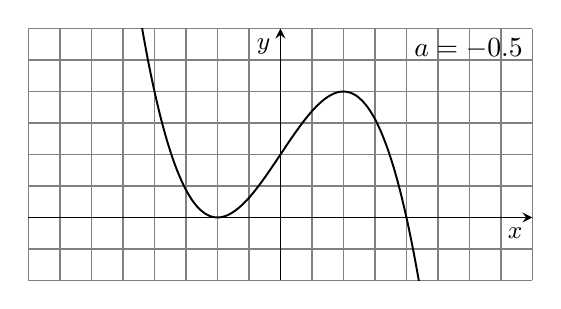
\begin{tikzpicture}[scale=0.800]
        % grid
        \draw[draw=black!50!white] (-4.000, -1.000) grid[step=0.5] (4.000, 3.000);
        % x-axis
        \draw[line width=0.6pt, ->, >=stealth] (-4.000, 0) -- (4.000, 0) node[below left] {\small$x$};
        % y-axis
        \draw[line width=0.6pt, ->, >=stealth] (0, -1.000) -- (0, 3.000) node[below left] {\small$y$};
        % function: f(x)=-\num{0.5}x^{3}+\num{1.5}x+\num{1}
        \begin{scope}[line width=0.7pt]
          \clip (-4.000, -1.000) rectangle (4.000, 3.000);
          \draw plot[smooth] coordinates
          {
            ( -4.000,   6.000) ( -3.900,   6.000) ( -3.800,   6.000)
            ( -3.700,   6.000) ( -3.600,   6.000) ( -3.500,   6.000)
            ( -3.400,   6.000) ( -3.300,   6.000) ( -3.200,   6.000)
            ( -3.100,   6.000) ( -3.000,   6.000) ( -2.900,   6.000)
            ( -2.800,   6.000) ( -2.700,   6.000) ( -2.600,   5.888)
            ( -2.500,   5.062) ( -2.400,   4.312) ( -2.300,   3.633)
            ( -2.200,   3.024) ( -2.100,   2.480) ( -2.000,   2.000)
            ( -1.900,   1.579) ( -1.800,   1.216) ( -1.700,   0.906)
            ( -1.600,   0.648) ( -1.500,   0.438) ( -1.400,   0.272)
            ( -1.300,   0.148) ( -1.200,   0.064) ( -1.100,   0.015)
            ( -1.000,   0.000) ( -0.900,   0.014) ( -0.800,   0.056)
            ( -0.700,   0.122) ( -0.600,   0.208) ( -0.500,   0.312)
            ( -0.400,   0.432) ( -0.300,   0.564) ( -0.200,   0.704)
            ( -0.100,   0.851) (  0.000,   1.000) (  0.100,   1.150)
            (  0.200,   1.296) (  0.300,   1.436) (  0.400,   1.568)
            (  0.500,   1.688) (  0.600,   1.792) (  0.700,   1.879)
            (  0.800,   1.944) (  0.900,   1.986) (  1.000,   2.000)
            (  1.100,   1.984) (  1.200,   1.936) (  1.300,   1.851)
            (  1.400,   1.728) (  1.500,   1.562) (  1.600,   1.352)
            (  1.700,   1.093) (  1.800,   0.784) (  1.900,   0.420)
            (  2.000,   0.000) (  2.100,  -0.481) (  2.200,  -1.024)
            (  2.300,  -1.634) (  2.400,  -2.312) (  2.500,  -3.062)
            (  2.600,  -3.888) (  2.700,  -4.000) (  2.800,  -4.000)
            (  2.900,  -4.000) (  3.000,  -4.000) (  3.100,  -4.000)
            (  3.200,  -4.000) (  3.300,  -4.000) (  3.400,  -4.000)
            (  3.500,  -4.000) (  3.600,  -4.000) (  3.700,  -4.000)
            (  3.800,  -4.000) (  3.900,  -4.000) (  4.000,  -4.000)
          };
        \end{scope}
        \node[below left] at (4,3) {$a=\num{-0.5}$};
      \end{tikzpicture}
      \hspace{1cm}
      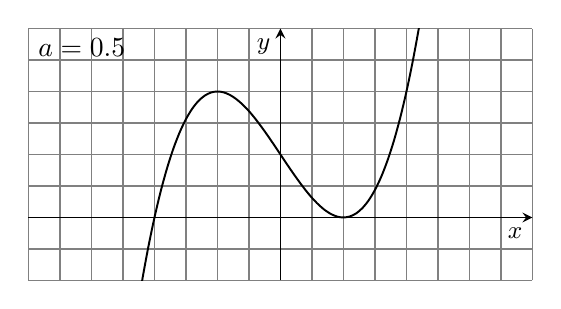
\begin{tikzpicture}[scale=0.800]
        % grid
        \draw[draw=black!50!white] (-4.000, -1.000) grid[step=0.5] (4.000, 3.000);
        % x-axis
        \draw[line width=0.6pt, ->, >=stealth] (-4.000, 0) -- (4.000, 0) node[below left] {\small$x$};
        % y-axis
        \draw[line width=0.6pt, ->, >=stealth] (0, -1.000) -- (0, 3.000) node[below left] {\small$y$};
        % function: f(x)=\num{0.5}x^{3}-\num{1.5}x+\num{1}
        \begin{scope}[line width=0.7pt]
          \clip (-4.000, -1.000) rectangle (4.000, 3.000);
          \draw plot[smooth] coordinates
          {
            ( -4.000,  -4.000) ( -3.900,  -4.000) ( -3.800,  -4.000)
            ( -3.700,  -4.000) ( -3.600,  -4.000) ( -3.500,  -4.000)
            ( -3.400,  -4.000) ( -3.300,  -4.000) ( -3.200,  -4.000)
            ( -3.100,  -4.000) ( -3.000,  -4.000) ( -2.900,  -4.000)
            ( -2.800,  -4.000) ( -2.700,  -4.000) ( -2.600,  -3.888)
            ( -2.500,  -3.062) ( -2.400,  -2.312) ( -2.300,  -1.633)
            ( -2.200,  -1.024) ( -2.100,  -0.480) ( -2.000,   0.000)
            ( -1.900,   0.421) ( -1.800,   0.784) ( -1.700,   1.094)
            ( -1.600,   1.352) ( -1.500,   1.562) ( -1.400,   1.728)
            ( -1.300,   1.852) ( -1.200,   1.936) ( -1.100,   1.985)
            ( -1.000,   2.000) ( -0.900,   1.986) ( -0.800,   1.944)
            ( -0.700,   1.878) ( -0.600,   1.792) ( -0.500,   1.688)
            ( -0.400,   1.568) ( -0.300,   1.436) ( -0.200,   1.296)
            ( -0.100,   1.149) (  0.000,   1.000) (  0.100,   0.850)
            (  0.200,   0.704) (  0.300,   0.564) (  0.400,   0.432)
            (  0.500,   0.312) (  0.600,   0.208) (  0.700,   0.121)
            (  0.800,   0.056) (  0.900,   0.014) (  1.000,   0.000)
            (  1.100,   0.016) (  1.200,   0.064) (  1.300,   0.149)
            (  1.400,   0.272) (  1.500,   0.438) (  1.600,   0.648)
            (  1.700,   0.907) (  1.800,   1.216) (  1.900,   1.580)
            (  2.000,   2.000) (  2.100,   2.481) (  2.200,   3.024)
            (  2.300,   3.634) (  2.400,   4.312) (  2.500,   5.062)
            (  2.600,   5.888) (  2.700,   6.000) (  2.800,   6.000)
            (  2.900,   6.000) (  3.000,   6.000) (  3.100,   6.000)
            (  3.200,   6.000) (  3.300,   6.000) (  3.400,   6.000)
            (  3.500,   6.000) (  3.600,   6.000) (  3.700,   6.000)
            (  3.800,   6.000) (  3.900,   6.000) (  4.000,   6.000)
          };
        \end{scope}
        \node[below right] at (-4,3) {$a=\num{0.5}$};
      \end{tikzpicture}
    \end{center}
    %printf("\\begin{center}\n");
    %a = -0.5;
    %f = [a 0 -3*a 1];
    %mypolyplot(f, -4, 4, -1, 3, 0.1, 0.8);
    %printf("\\hspace{1cm}\n");
    %a = 0.5;
    %f = [a 0 -3*a 1];
    %mypolyplot(f, -4, 4, -1, 3, 0.1, 0.8);
    %printf("\\end{center}\n");
    % </OUTCOME>
  \fi
\end{exercise}
